\subsection{Subpaso 1-A: Iniciar sanción para el solicitante}
	Para acceder a sancionar a un solicitante se da click en el botón
	 \textbf{Generar Prestamos} localizado en la parte izquierda del menú
	
	\begin{figure}[hbtp]

	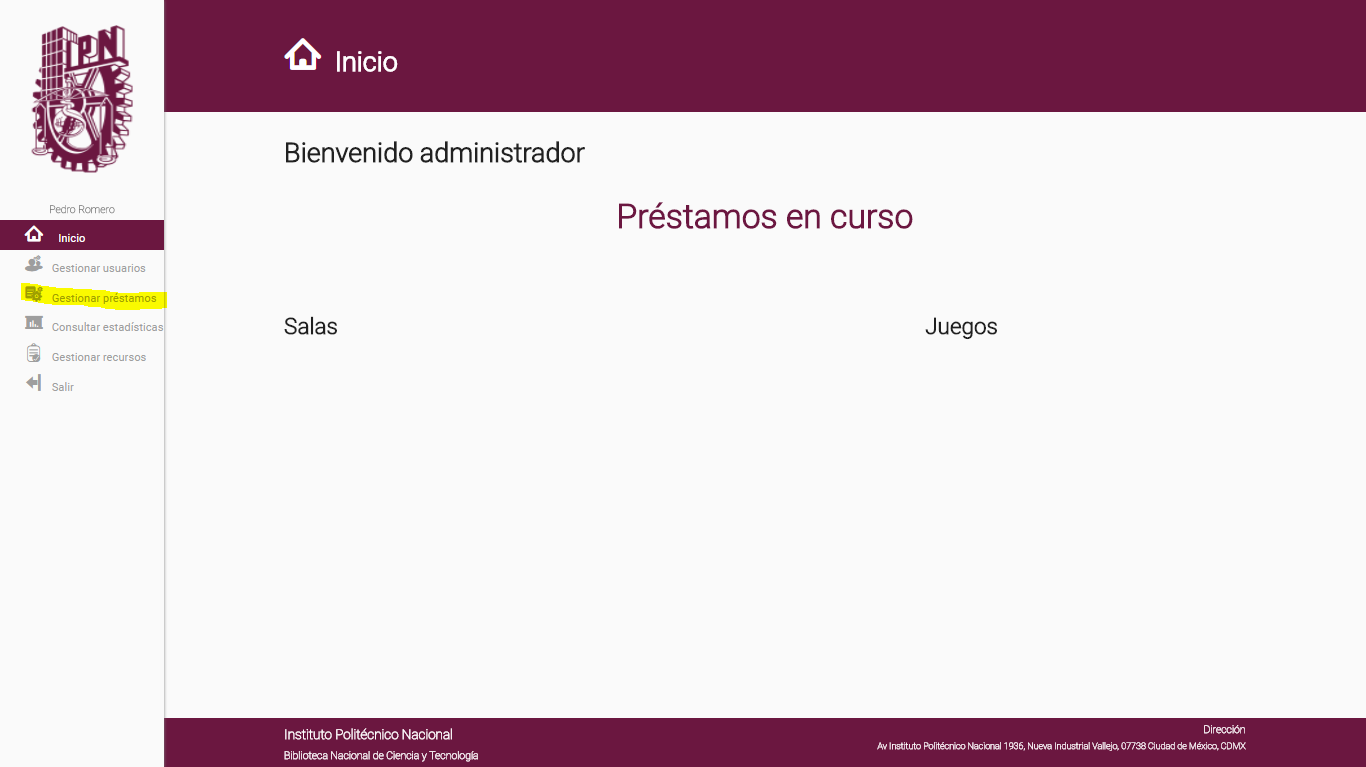
\includegraphics[scale=0.3]{images/Interfaz/IUGS07_bienvenida.PNG}
	\caption{Bienvenida}
	\end{figure}
\subsection{Subpaso 1-B: Buscar solicitante a sancionar}
\begin{itemize}


	\item Para poder buscar a un solicitante se tienen las siguientes dos maneras 
	\begin{enumerate}
		\item Buscar por identificador 
		\begin{figure}[hbtp]
	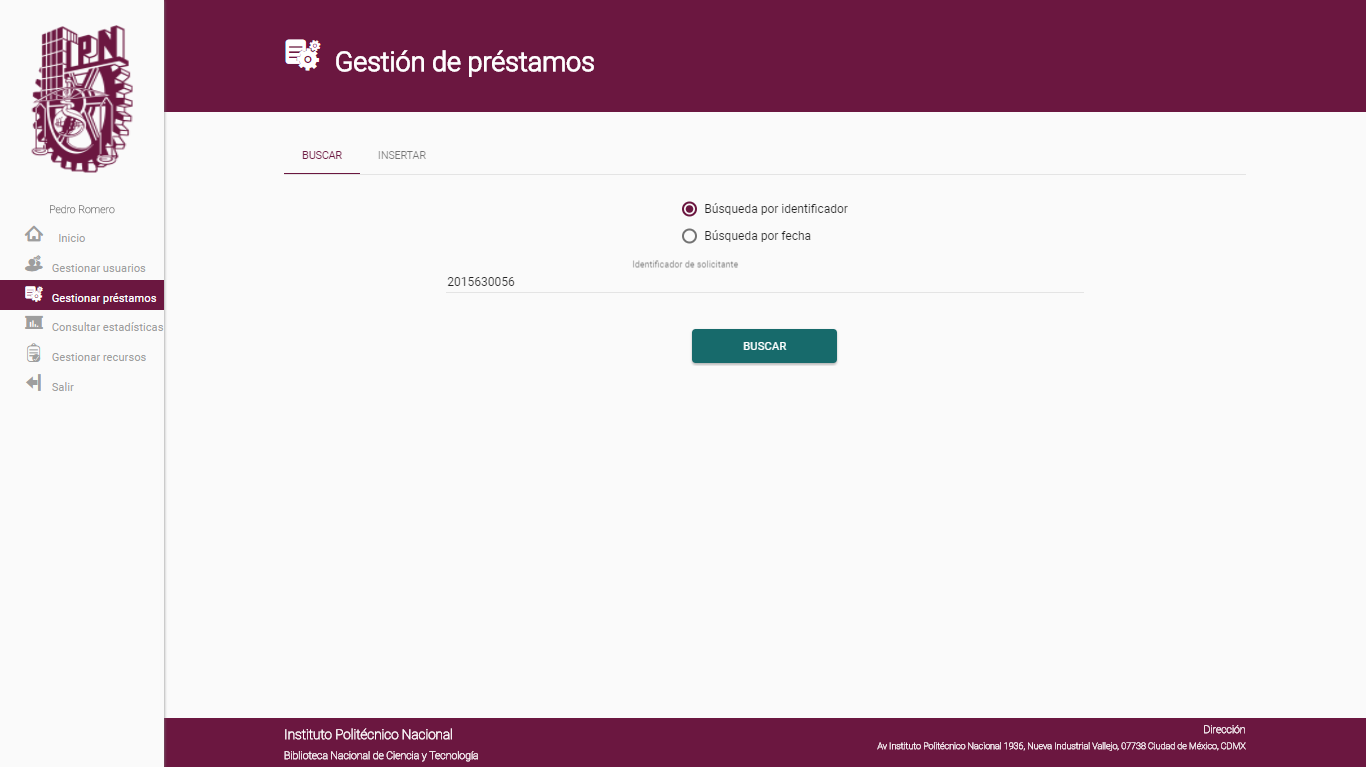
\includegraphics[scale=0.3]{images/Interfaz/IUGS07_gestionarPrestamoID.PNG}
	\caption{Gestionar Préstamo con Identificador}
	\end{figure}
	
	\item Buscar por fecha
	\begin{figure}[hbtp]
	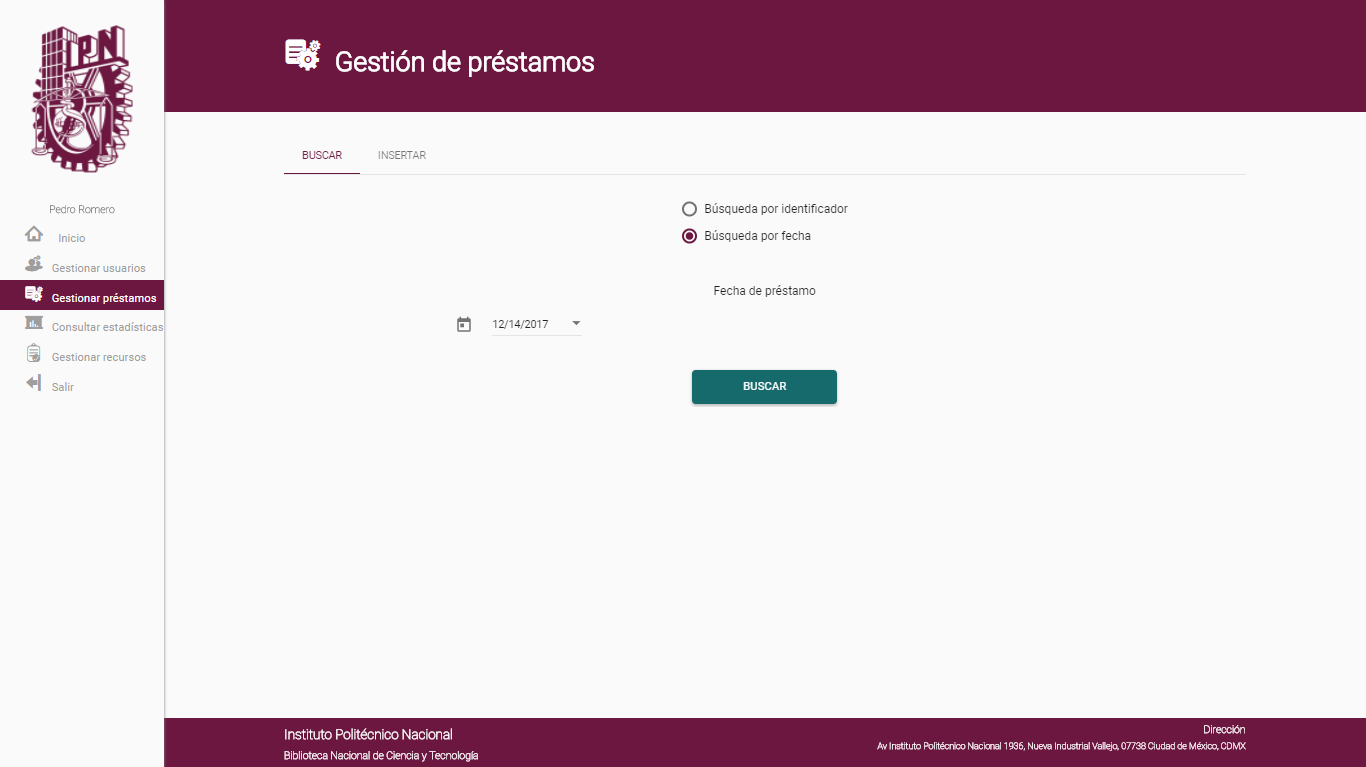
\includegraphics[scale=0.3]{images/Interfaz/IUGS07_gestionarPrestamoFecha.PNG}
	\caption{Gestionar Préstamo con Fecha}
	\end{figure}
	
	\end{enumerate}
	\item Presionar el botón \textbf{Buscar}
	
	\begin{figure}[hbtp]
	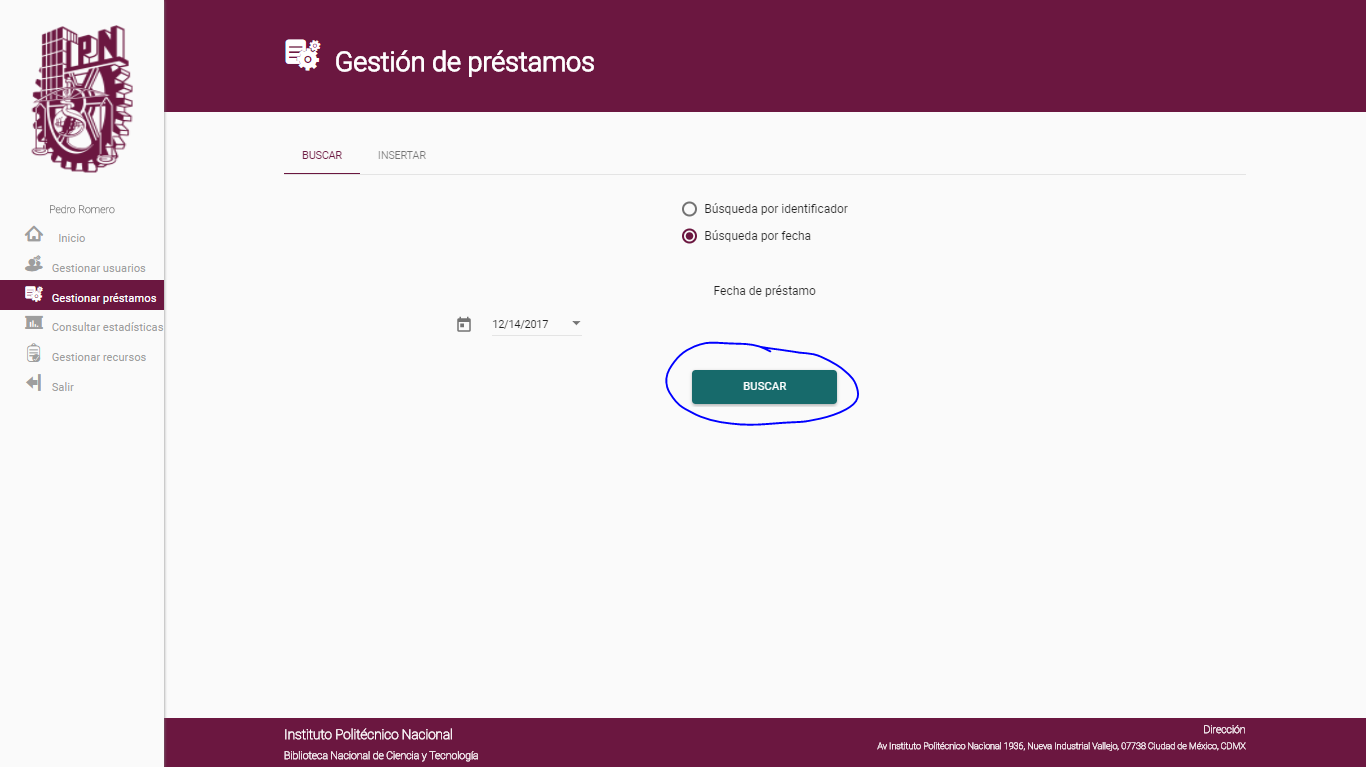
\includegraphics[scale=0.3]{images/Interfaz/IUGS07_gestionarPrestamoBuscar.PNG}
	\caption{Gestionar Préstamo Botón Buscar}
	\end{figure}
\end{itemize}